\chapter{Observations}
We observed data from both the serial monitor of the Arduino IDE, as well as from the graph in processing. Since we wanted our device to give the best results as quickly as possible, we decided to calibrate it.
\begin{figure}[H]
	\vfill
	\centering
	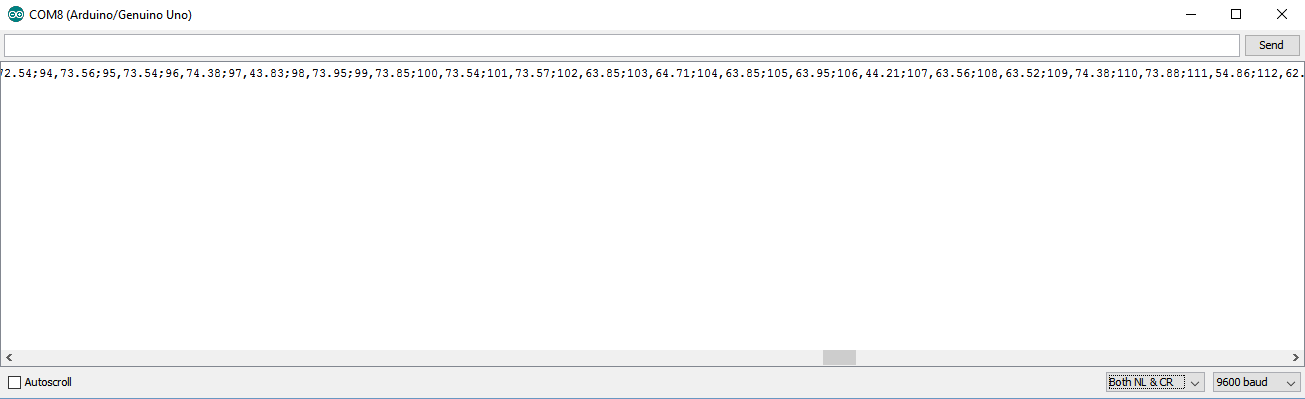
\includegraphics[width=0.7\textwidth]{../Files/sermon}
	\caption{Data Observed in the Serial Monitor of the Arduino IDE}  \label{fig:sermon}
\end{figure}
\section{Calibration}
\subsection{Calibration of Measurements}
We realised that actual measurements of distance/count/width of an object placed in the vicinity of the apparatus were different from the ones provided by our device. Hence, we proceeded to calibrate each part of our device that was capable of taking a measurement.\\

The quantities that were measured in our project before going for any further calculations were: \underline{Angle} and \underline{Distance}. The rest were only obtained by playing around with these two main quantities. Hence, we needed them to be as accurate as possible.\\

We did not notice any error in the value of angle that the motor was rotating to, hence we did not have to do any sort of calibration for it.\\

To calibrate the distance, we placed several objects at fixed distances from the sensor on a white chart paper, with values of distances marked on it with the help of a ruler. We then made measurements keeping the sensor still, and made an adjustment to the formula in the code by observing the multiplication factor that needed to be introduced into the previous formula in order to get the correct values. Hence, the formula was changed from "duration/58" to "duration/58.2".\\
\begin{figure}[H]
	\vfill
	\centering
	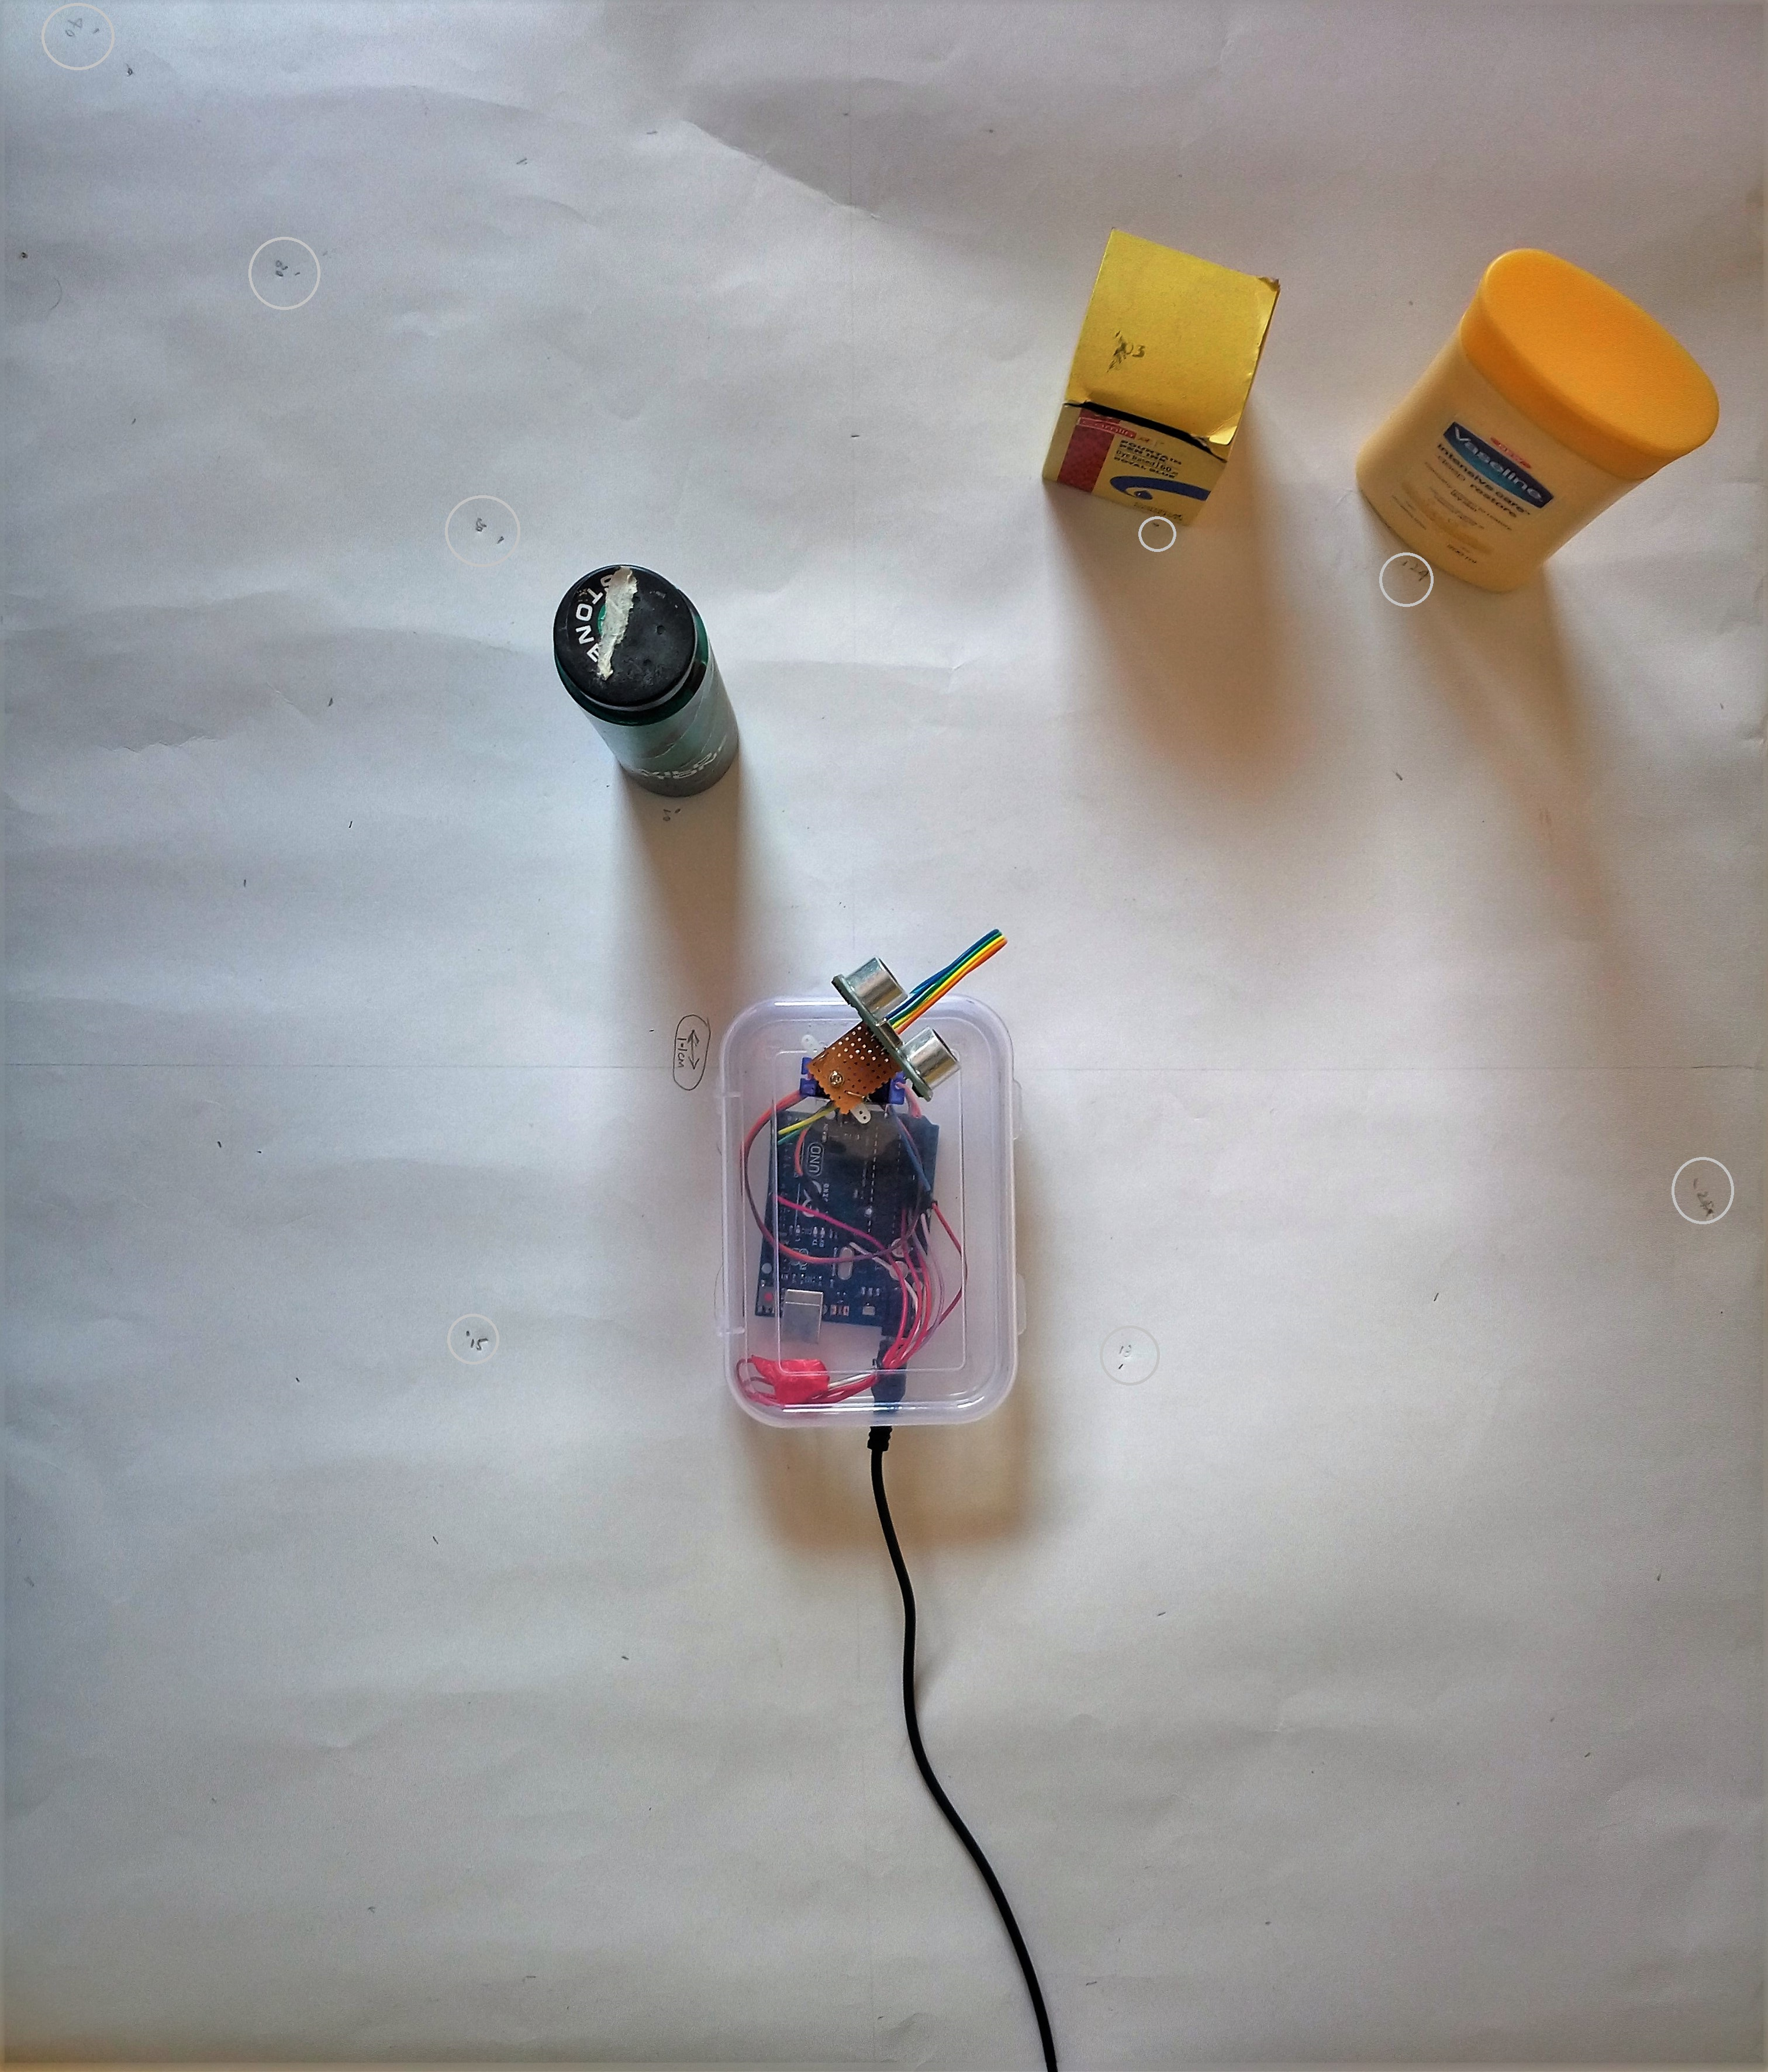
\includegraphics[width=\textwidth]{../Files/cabri.jpg}
	\caption{Calibration on chart paper with marked distances}  \label{fig:sermon}
\end{figure}
\subsection{Optimising Speed}
We wanted to optimise our device to work as quickly as possible, without affecting normal execution of the program. So we optimised our code, considering the delays in physical movement, time periods of recieved/transmitted waves and time taken to process the data.\\
We took into account the several delays introduced in the code, along with the delay in rotation of the motor(specified by its speed given in its datasheet, tested to be accurate) and delay in calculation of distance. Accordingly, we minimised each of the values given as arguments to the \begin{verbatim}delay()\end{verbatim} function used at different parts of the Arduino code, to the safest least value possible. Each of the delays with descriptions can be observed in the Arduino code given with comments in Appendix \ref{ch:appAlabel}
\section{Graphs}
We obtained the following [error vs. position] graphs for three different kinds of objects kept in front of the sensor. In each case, we noted down values for both the sensor being stationary, and rotating. The three different kinds of objects were
\begin{itemize}
	\item Object1 = Hollow plastic bottle (width=6cm)
	\item Object2 = Solid DC battery (width=3cm)
	\item Object3 = Metallic pen (width=0.8cm)
\end{itemize}

\begin{figure}[H]
	\vfill
	\centering
	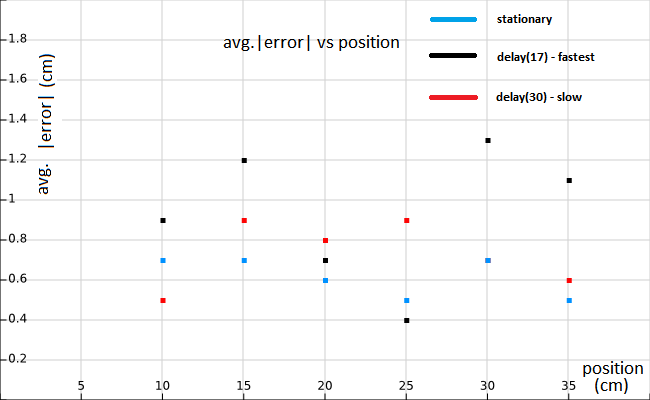
\includegraphics[width=0.8\textwidth]{../Files/save12}
	\caption{Object1-avg.|error| vs position} 
\end{figure}
\begin{figure}[H]
	\vfill
	\centering
	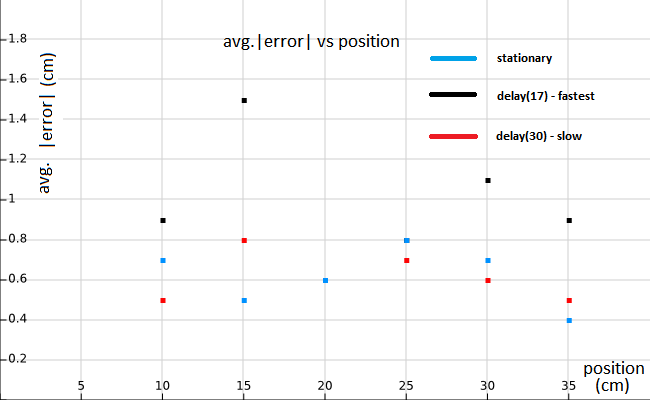
\includegraphics[width=0.8\textwidth]{../Files/save21}
	\caption{Object2-avg.|error| vs position} 
\end{figure}
\begin{figure}[H]
	\vfill
	\centering
	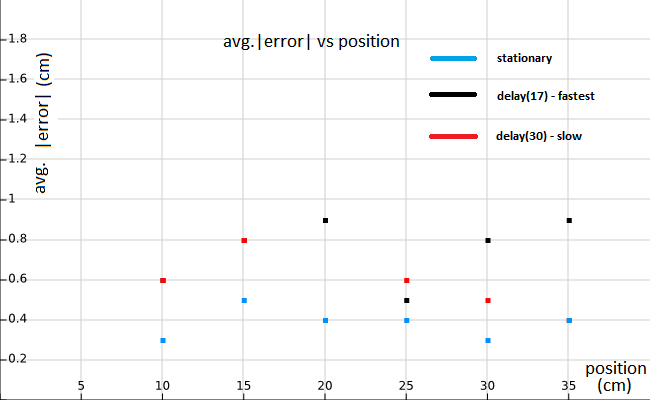
\includegraphics[width=0.8\textwidth]{../Files/save32}
	\caption{Object3-avg.|error| vs position}  
\end{figure}
\clearpage
Finally, we also plotted the error in data of width of object vs. position, which was something like this:
\begin{figure}[H]
	\vfill
	\centering
	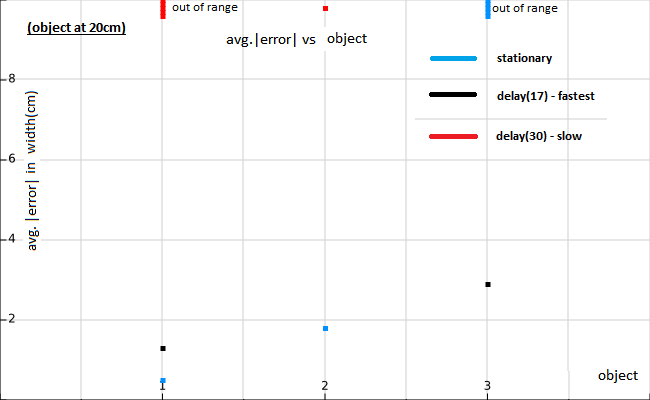
\includegraphics[width=\textwidth]{../Files/savew1}
	\caption{Object-wise avg.|error| in width at x=20cm} 
\end{figure}
\clearpage